They are a few reasons for finding the diamonds and not only the outer or inner part of the table.

\begin{itemize}
	\item The diamonds provide key knowledge about pixel to meter ratio.
	\item To be able to have the smallest ROI to search for the balls. Note that the only fixed length to find the exact playing field are from the diamonds to the cushion as mentioned in \ref{sec:rules}
	\item For possible later implementation of UI where diamonds act as buttons.
\end{itemize}

The diamonds have several properties that will be used when locating them. As written in the pool table specifications \ref{sec:rules} the diamonds have a few useful properties:

\begin{itemize}
	\item They must be located with the same distance of each other.
	\item The center of each diamond must be located 93.5 mm from the nose of the cushion.
	\item They may be round or diamond-shaped.
	\item They stand out from their surroundings.
\end{itemize}

The table are be found in the previous section\ref{sec:table-locate} and thereby making the search-region for the diamonds smaller. Also, within the table there are very few contours that could appear to be a diamonds, where as outside the table the environment is completely different from place to place.\\

For robustly locating the diamonds the following approach has been used:
\begin{enumerate}
	\item Convert captured image to grayscale.
	\item Make binary with adaptive threshold.
	\item Find contours and sort them by size
	\item Do step 1 to 3 for several images.
	\item Find the contours that remain at same position throughout the sequence.
\end{enumerate}

%MAKE FLOWCHART.

\textbf{Convert to grayscale and use adaptive threshold:}\\
The captured image will be converted into grayscale for further process where it is made binary with adaptive threshold. This will provide much more invariance to light in the different regions of the table. More can be read about adaptive threshold in section \ref{sec:table-locate}.\\

%Insert Image

\textbf{Find contours:}\\
The next step is to find the contours in the binary image and sort them by size. The contours are found by using OpenCV build in contour detection algorithm \cite{contour}.

This will return a list of contours in the image\ref{fig:allcontours}.

\begin{figure}[H]
\begin{center}
\leavevmode
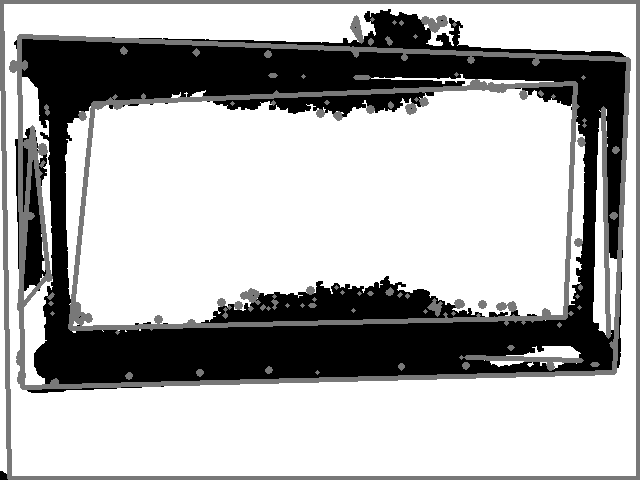
\includegraphics[width=0.5\textwidth]{images/allcontours.png}
\end{center}
\caption{All contours found in frame.}
\label{fig:allcontours}
\end{figure}

Many different contours are found as seen and therefore it is necessary to sort the contours based on their size and remove those that are outliers. A diamond should obey certain rules:

\begin{itemize}
	\item Size: The maximum diamond is [31.75 x 15.875 mm]. That is 0.0005 $m^2$. The smallest table is 3.5$m^2$. If the table completely fills up the frame the diamond can, at most, be $1/7000$ of the frame. By knowing the width and height of the image other contours above this size can be removed. Since the morphology operations changes the sizes the threshold is set at $1/3500$.
	\item The diamond is convex.
\end{itemize}

The area size used as reference is the median area of the list of contours. This should be approximately the area of a diamond. If the mean was used instead of the median a much larger value would be the reference, because of very big contours being found (in OpenCV implementation the image in itself is a contour).

The outcome is a list of possible diamonds.\\\\

\textbf{Find contours for a sequence of images:}\\
While testing, one of the major problems with finding the diamonds positions, was the noise introduced by various parameters (camera, lightning etc). The actual positions of the diamonds was found in every frame, but a lot of noise made found positions of diamonds elsewhere in the images. 
The noise changed from frame to frame.

Therefore, by using a sequence of images (video) and compare the positions found it is possible to eliminate the noise and only find the position of the diamonds.

Each time an image is processed the contours are saved in a list. When the decided number of images has been processed it is simply a process of comparing the lists and find the points that have not moved or at least have not moved very much.\\

\begin{figure}[H]
\begin{center}
\leavevmode
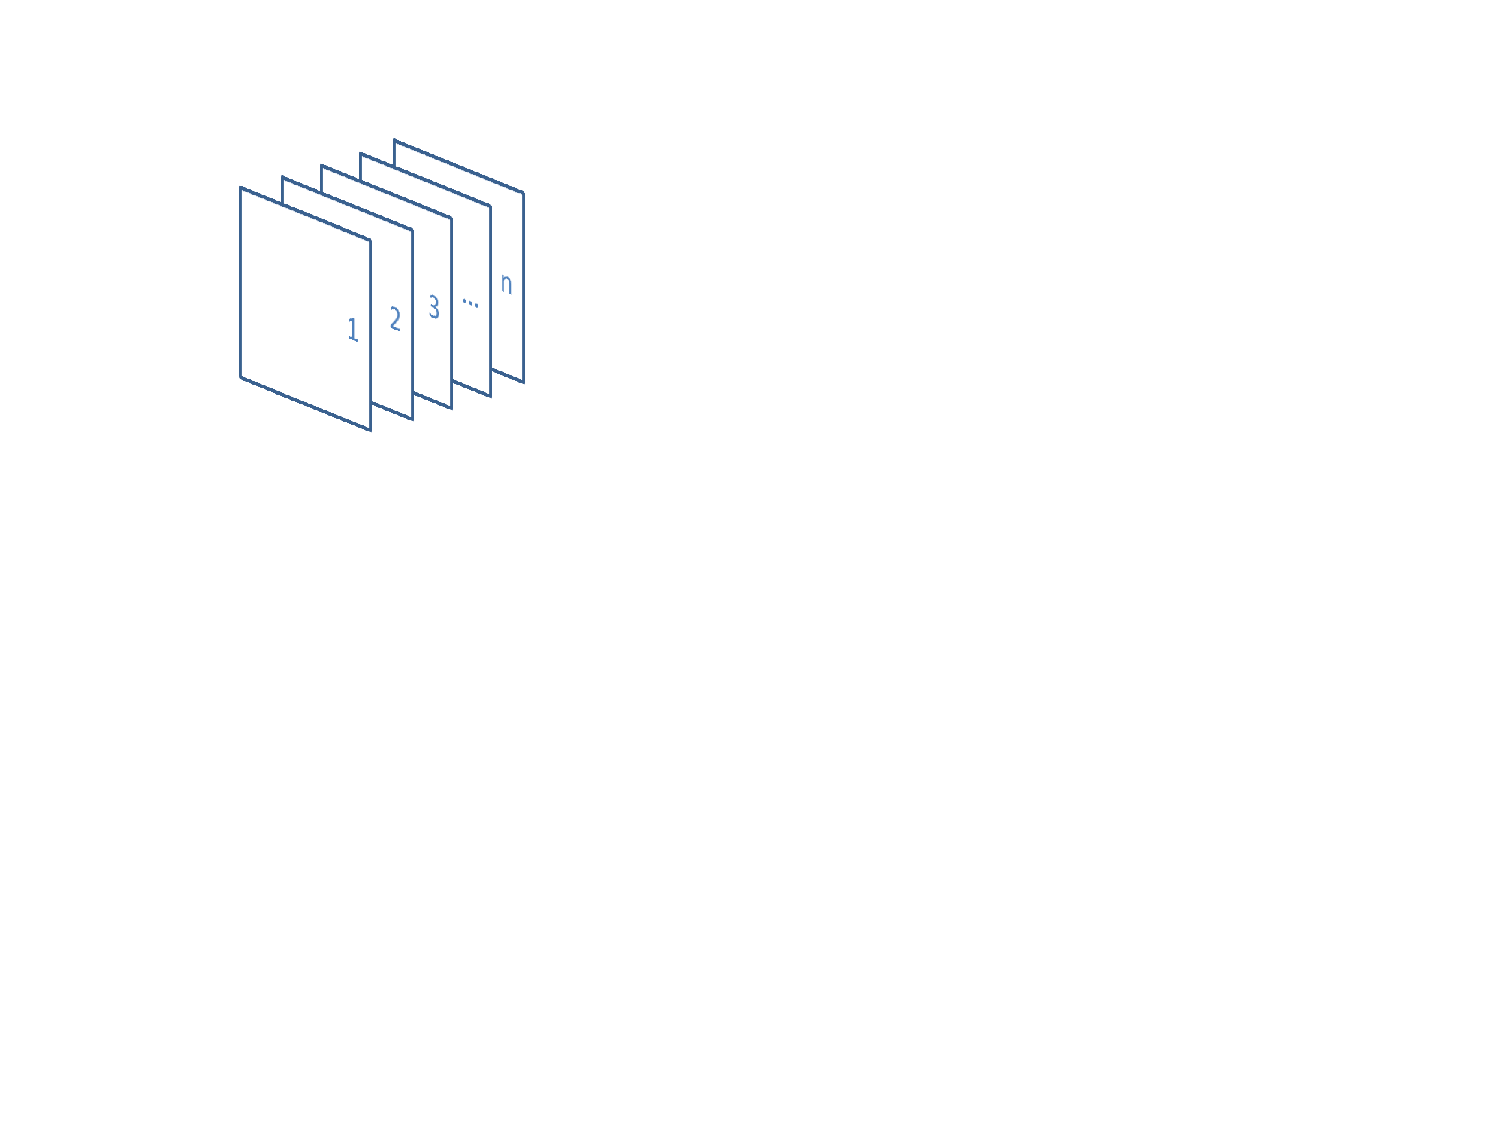
\includegraphics[width=0.5\textwidth]{images/image_seq_numbers.pdf}
\end{center}
\caption{Sequence of frames. The number of frames can be set as n.}
\label{fig:seq_img}
\end{figure}

\textbf{Find the contours that remain at same position throughout the sequence:}\\
A arbitrary point in the first frame is chosen. In all other frames the same position is searched for a contour. If this contour exists in every frame it is saved as a diamond. If it does not exist in every image it is not saved.

\begin{figure}[H]
\begin{center}
\leavevmode
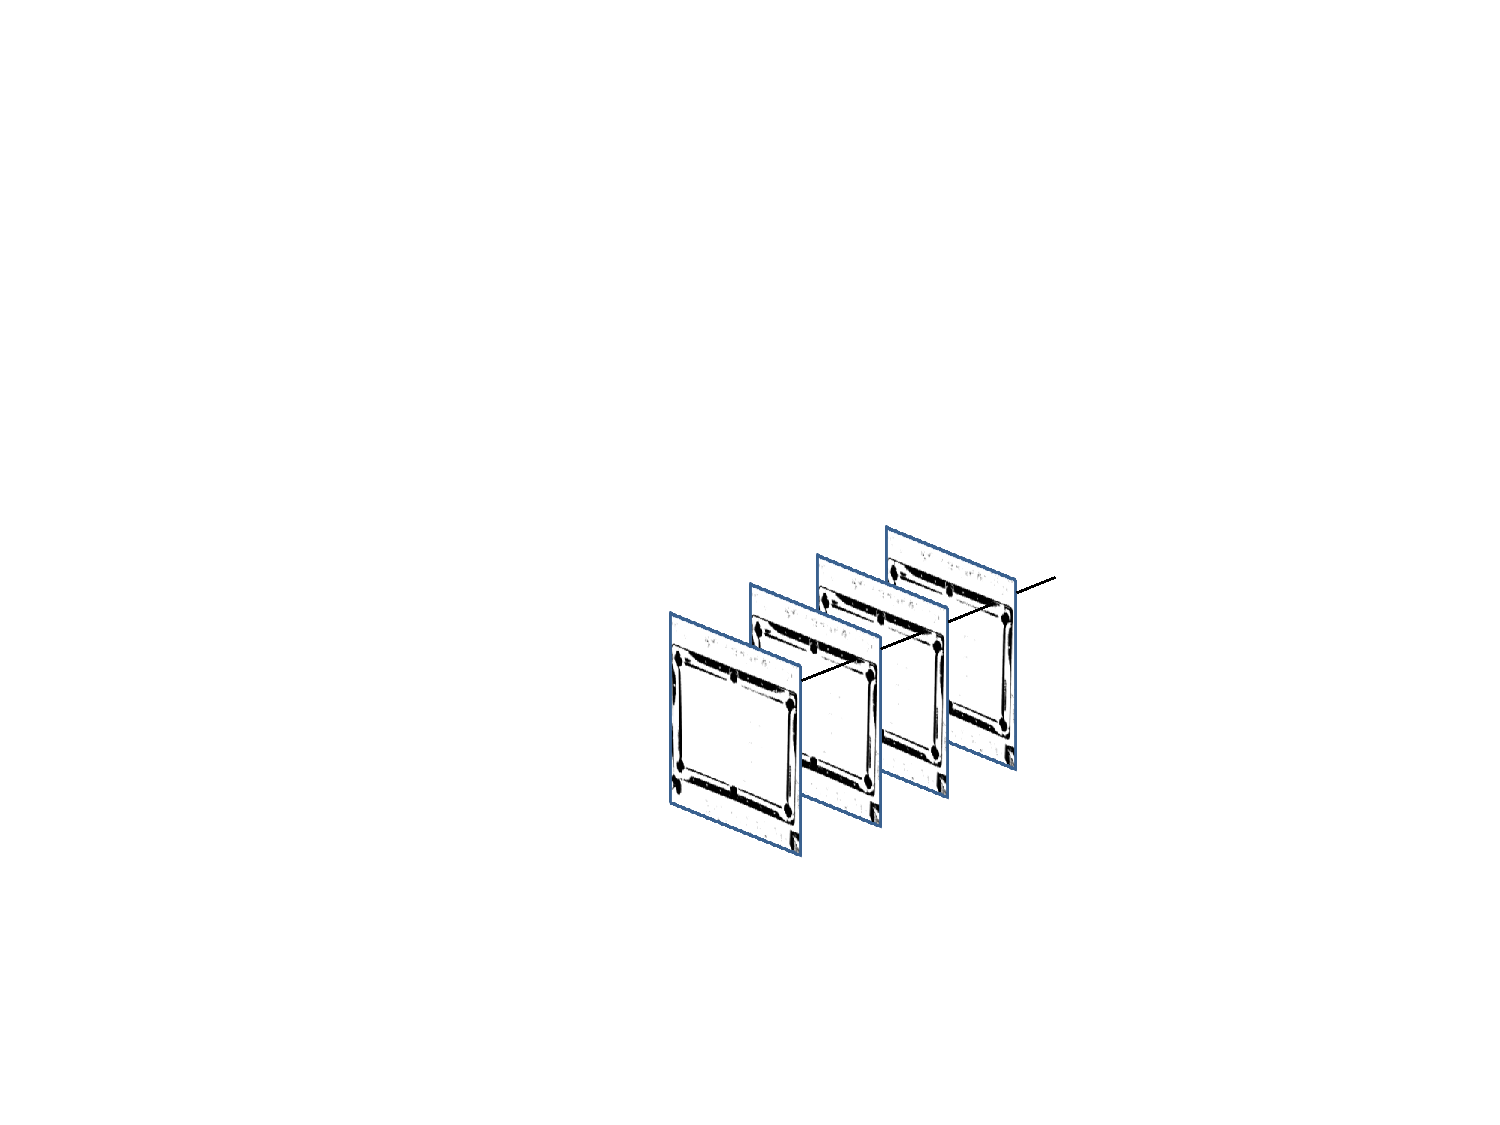
\includegraphics[width=0.5\textwidth]{images/image_seq_pool.pdf}
\end{center}
\caption{Searching for a contour in from the first frame in all other frames.}
\label{fig:seq_img_pool}
\end{figure}

